% Source: graduate-coursework/Prior_Semesters/Fa23/ELCT432/assignments/CA5P_Random_Bit_Generator/CA5.tex
% Description: PMF of Random Variable \(X\)

\documentclass[border=4pt]{standalone}
\usepackage{color}
\usepackage{courier}
\usepackage{graphicx}
\usepackage{tikz}

\definecolor{mygreen}{rgb}{0,0.6,0}
\definecolor{mygray}{rgb}{0.5,0.5,0.5}
\definecolor{mymauve}{rgb}{0.58,0,0.82}

\begin{document}
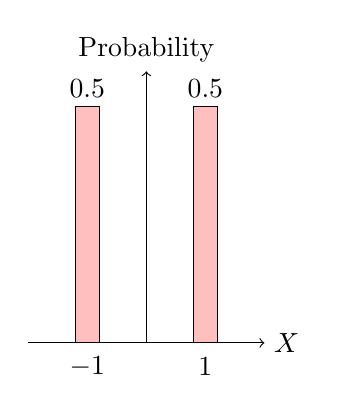
\begin{tikzpicture}[scale=1.5]
    \draw[->] (-1,0) -- (1,0) node[right] {\(X\)};
    \draw[->] (0,0) -- (0,2.3) node[above] {Probability};
    
    \foreach \x/\y in {-1/0.5, 1/0.5} {
      \draw[fill=pink] (\x*0.5-0.1,0) rectangle ++(0.2,\y*4);
      \node at (\x*0.5, \y*4.3) { \(\y\)};
    }
    
    \foreach \x/\y in {-1/-1, 1/1} {
      \node at (\x*0.5, -0.2) { \(\y\)};
    }
  \end{tikzpicture}
\end{document}
